\section{General Architecture}




\section{Schematics}
\subsection{Sampling-Channel}
\paragraph{Track-And-Hold-Amplifier}
Explain why better than Sample-And-Hold-Amplifier.
\paragraph{Delay Chip NB6L295}
Dual Channel Programmable Delay Chip.

\begin{itemize}[noitemsep]
	\item Two individual variable delay channels
	\item Dual Delay: minimal delay \SI{3.2}{\nano \second}
	\item Total Delay Range: \SI{3.2}{\nano \second} to \SI{8.8}{\nano \second} per Delay Channel
	\item \SI{11}{\pico \second} Increments in 511 steps
	\item \SI{100}{\pico \second} Typical Rise and Fall Times
\end{itemize}

\subsection{Clocking}
On Xilinx CLK104 add-on board the LMX2594 is used to generate additional, high-frequency clocks for the ADCs/DACs. $\rightarrow$ reuse in front-end card
\begin{figure}[tbh]
	\centering
	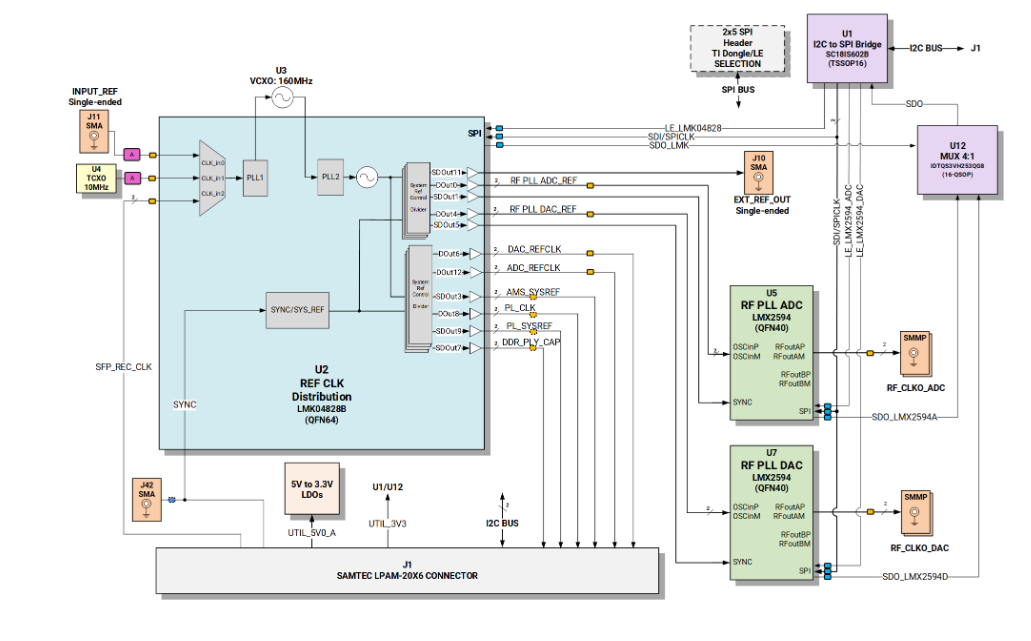
\includegraphics[width = 0.7\textwidth]{chap/04-work/img/clk104}
	\caption{CLK104 Add-on board clocking scheme}
	\label{fig:clk104}
\end{figure}

\begin{figure}[tbh]
	\centering
	\includegraphics[height = 0.3\textwidth, width = 0.55\textwidth]{chap/04-work/img/pll_tsMode.tikz}
	\caption{Clocking scheme on front-end card}
	\label{fig:clocking}
\end{figure}


\begin{figure}[tbh]
	\centering
	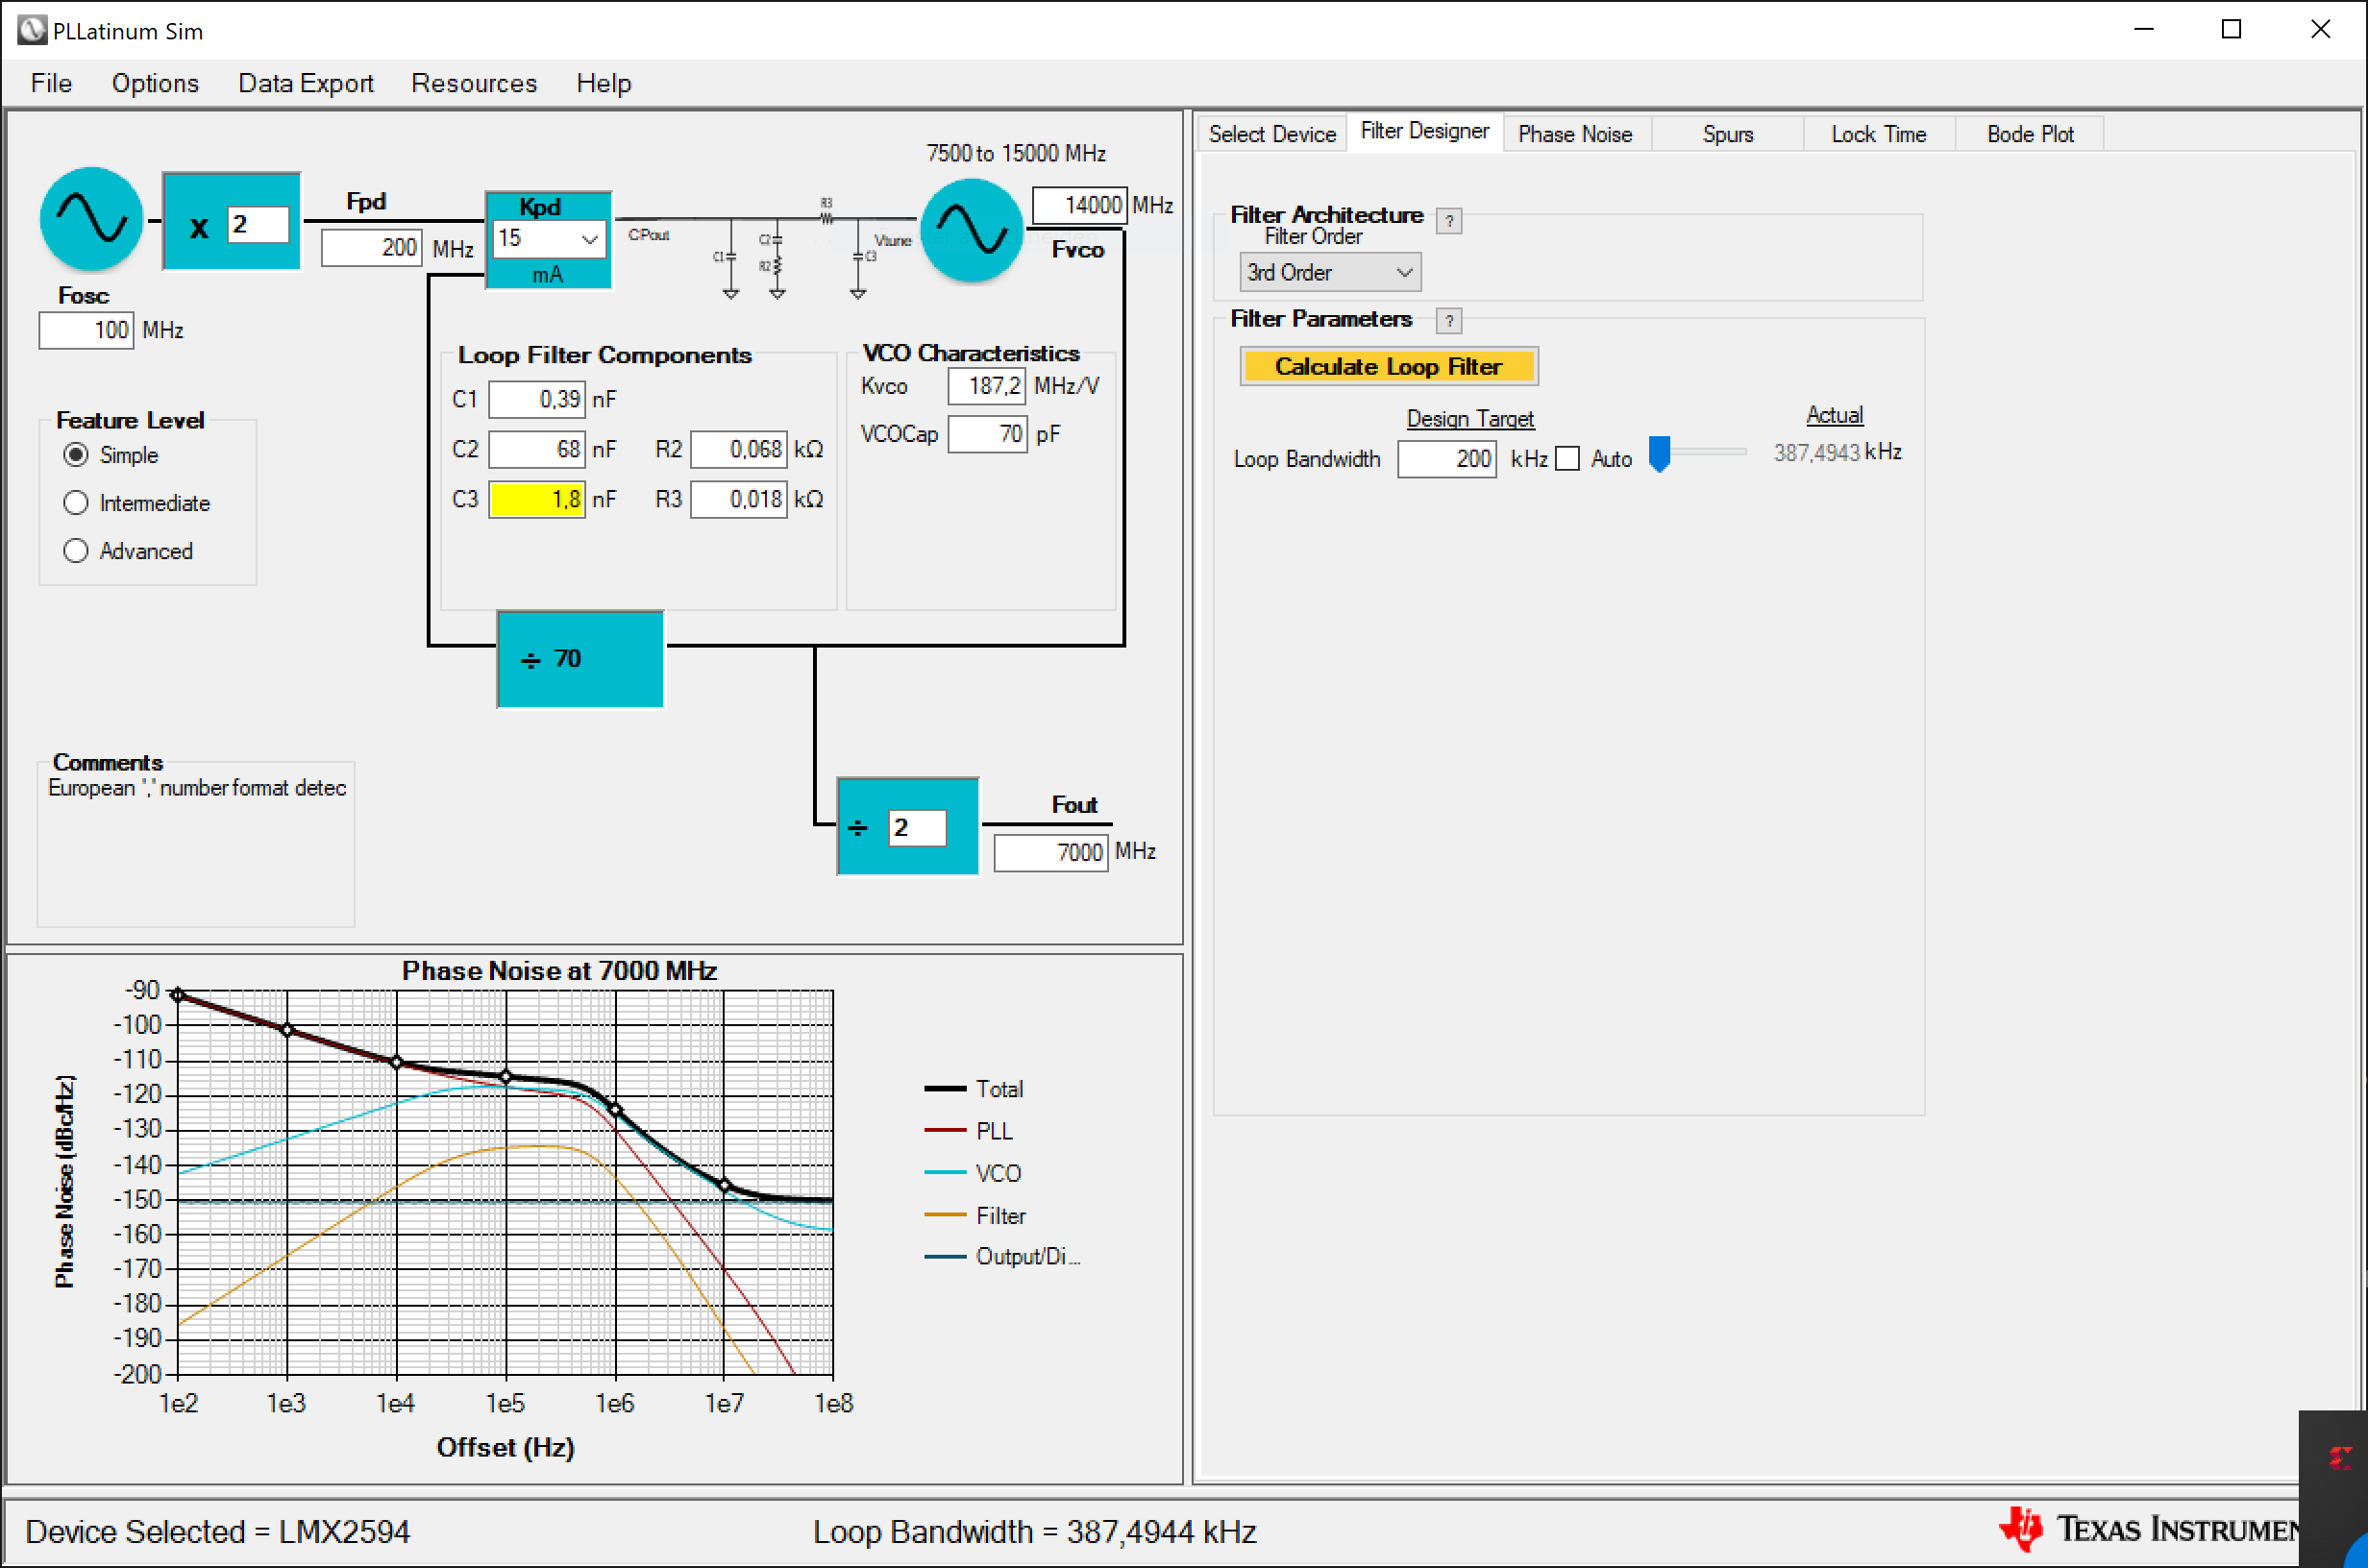
\includegraphics[width = 0.7\textwidth]{chap/04-work/img/pll.png}
	\caption{Placeholder}
	\label{fig:pll}
\end{figure}



\subsection{Power Supply}
For the Track-And-Hold amplifiers a new power supply unit -- the ADP1741 (Analog Devices) -- should be used. It is necessary to think about the amount of power supply chips needed. As a rule of thumb, the power supply should provide twice the maximum power needed by the components it drives. The power consumption/maximum current for the respective components on the THERESA board is listed in \autoref{tab:kapturecomp}. 
\begin{table}[tbh]
	\caption{Power consumption of components on the board}
	\label{tab:kapturecomp}
	\begin{minipage}{\textwidth}
		\centering
		\begin{tabularx}{\textwidth}{XSSSSS}
			\toprule
			\textbf{Component} & \textbf{$V_{cc}$ (\SI{}{\volt})} & \textbf{$I_{max}$ (\SI{}{\ampere})} & \textbf{$P_{max}$ (\SI{}{\watt})} & $\#_{parts}$ & \textbf{$I_{tot}$}\footnote{for 16 ADCs} (\SI{}{\ampere})\\
			\midrule
			HMC5649 (T/H-Amplifier) 	& 2	  	& 0.221 	 & 0.442 & 16 & 3.536\\
			& -5  	& -0.242 & 1.21 &  & 3.872\\
			HMC856 (Delay) 			& -3.3	& 0.185 & -0.611 & 16 & 2.96\\
			HMC987LP5E (Fan-Out) 	& 3.3 	& 0.234\footnote{All Outputs and RF-Buffer} & 0.772 & 2 & 0.468\\
			LMC0480 (PLL) 			& 3.3 	& 0.590\footnote{All CLKs} & 1.947 & 1 & 0.590\\
			VCXO 					& 3.3 	& 0.03 & 0.198 & 1 & 0.03\\
			\bottomrule
		\end{tabularx}
	\end{minipage}
\end{table}

The maximal current which the ADP1741 can provide @\SI{2}{\volt} is \SI{2}{\ampere}. This means, with one Track-And-Hold amplifier requiring a maximal current of \SI{0.221}{\ampere}, one ADP1741 can handle four units according to the rule mentioned beforehand ($I_{max\_ADP1741} = \SI{2}{\ampere} > 2 * I_{tot}, I_{tot} = 4 \times \SI{0.221}{\ampere} =  \SI{0.884}{\ampere}$).



\section{Layout}

\subsection{Floor Planning}
\subsection{Transmission lines}
\paragraph{RF/Microwave Design Basics}

\paragraph{Surface Coplanar Waveguide with Ground}  
\begin{figure}[!htbp]
	\centering
	\begin{tikzpicture}
		\filldraw[color=black, fill=black] (0,0.7) rectangle ++(9,0.3) node[pos=.5](gnd){};
		\filldraw[color=black, fill=gray!20] (0,1) rectangle ++(9,2) node[pos=.5]{\(\varepsilon_r\)};
		\filldraw[color=black, fill=black] (0,3) rectangle ++(2,.2) node[pos=.5](GND1){};
		\filldraw[color=black, fill=black] (3,3) rectangle ++(1,.2) node[pos=.5](cond1){};
		\filldraw[color=black, fill=black] (5,3) rectangle ++(1,.2) node[pos=.5](cond2){};
		\filldraw[color=black, fill=black] (7,3) rectangle ++(2,.2) node[pos=.5](GND2){};
		\draw[>=triangle 45, <->] (-0.5,1) -- (-0.5,3) node[pos=.5,anchor=east](){\(h\)};
		\draw[>=triangle 45, <->] (2,4) -- ++(1,0) node[pos=.5,anchor=south](){\(d\)};
		\draw[>=triangle 45, <->] (3,3.8) -- ++(1,0) node[pos=.5,anchor=south](){\(w\)};
		\draw[>=triangle 45, <->] (4,3.6) -- ++(1,0) node[pos=.5,anchor=south](){\(s\)};
		
		\draw[>=triangle 45, ->] (10,4) -- (10,3.2) node[pos=.5,anchor=west](){\(t\)};
		\draw[>=triangle 45, ->] (10,2.2) -- (10,3) node[pos=.5,anchor=west](){};
		
		\draw[decorate,decoration={zigzag,segment length=10mm, amplitude=1mm},double, double distance = 8.9pt, white] (9,0) -- (9,4);
		\draw[decorate,decoration={zigzag,segment length=10mm, amplitude=1mm},double, double distance = 8pt, white] (0,-0.5) -- (0,4);
		\draw[dashed] (0.1,1) -- (-1,1);
		\draw[dashed] (0.2,3) -- (-1,3);
		\draw[dashed] (8,3.2) -- (10,3.2);
		\draw[dashed] (8,3) -- (10,3);
		
	\end{tikzpicture}
	\caption{Edge-Coupled Coplanar Waveguide}
	\label{fig:eccw_geometry}
\end{figure}





\begin{figure}[!htbp]
	\centering
	\begin{tikzpicture}
		
		\filldraw[color=black, fill=black] (0,0.7) rectangle ++(9,0.3) node[pos=.5](gnd){};
		\filldraw[color=black, fill=gray!20] (0,1) rectangle ++(9,2) node[pos=.5]{\(\varepsilon_r\)};
		\filldraw[color=black, fill=black] (0,3) rectangle ++(2,.2) node[pos=.5](GND1){};
		\filldraw[color=black, fill=black] (3.5,3) rectangle ++(2,.2) node[pos=.5](cond1){};
		\filldraw[color=black, fill=black] (7,3) rectangle ++(2,.2) node[pos=.5](GND2){};
		\draw[>=triangle 45, <->] (3.5,3.4) -- ++(2,0) node[pos=.5,anchor=south](){\(a\)};
		\draw[>=triangle 45, <->] (2,3.8) -- ++(5,0) node[pos=.5,anchor=south](){\(b\)};
		
		\draw[>=triangle 45, <->] (-0.5,1) -- (-0.5,3) node[pos=.5,anchor=west](){\(h\)};
		\draw[>=triangle 45, ->] (10,4) -- (10,3.2) node[pos=.5,anchor=west](){\(t\)};
		\draw[>=triangle 45, ->] (10,2.2) -- (10,3) node[pos=.5,anchor=west](){};
		
		\draw[decorate,decoration={zigzag,segment length=10mm, amplitude=1mm},double, double distance = 8.9pt, white] (9,0) -- (9,4);
		\draw[decorate,decoration={zigzag,segment length=10mm, amplitude=1mm},double, double distance = 8pt, white] (0,-0.5) -- (0,4);
		\draw[dashed] (0.1,1) -- (-1,1);
		\draw[dashed] (0.2,3) -- (-1,3);
		
		\draw[dashed] (7,3.2) -- (10,3.2);
		\draw[dashed] (8,3) -- (10,3);
		
	\end{tikzpicture}
	\caption{Coplanar Waveguide with Ground}
	\label{fig:microstrip_geometry}
\end{figure}



\begin{figure}[tbh]
	\centering
	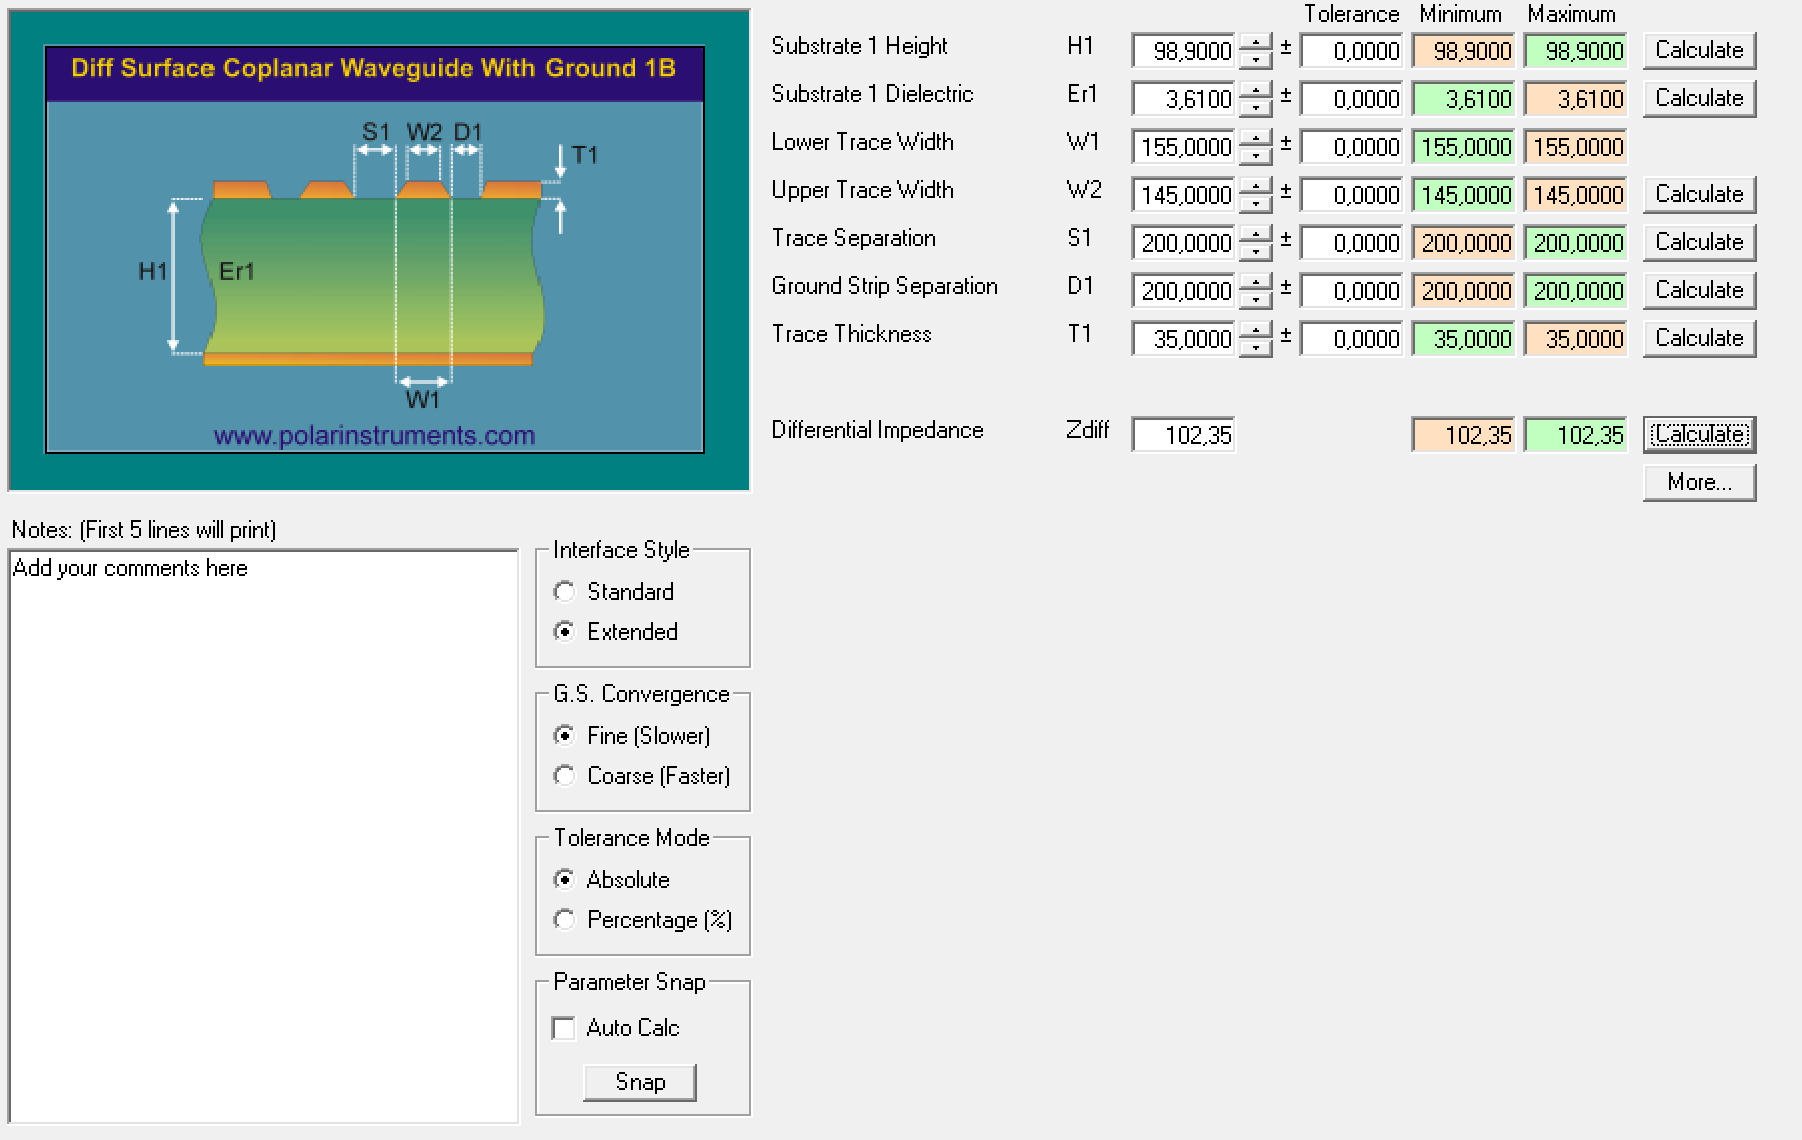
\includegraphics[width = 0.8\textwidth]{chap/04-work/img/polaris}
	\caption{Polaris Solver}
	\label{fig:polaris}
\end{figure}

\begin{figure}[tbh]
	\centering
	\includegraphics[width = \textwidth, height = 0.5\textwidth]{chap/04-work/img/megtron_diff_bottom_d1_vs_s1.tikz}
	\caption{Test Graph}
	\label{fig:megtron}
\end{figure}


\section{Production}